\documentclass[10pt,twocolumn]{article}

% ---- venue-specific: font + page geometry (generic two-column build) ----
\usepackage[utf8]{inputenc}
\usepackage[T1]{fontenc}
\usepackage{mathptmx}
\usepackage[margin=0.85in]{geometry}
\usepackage{lineno}

% ---- shared style: packages, integrity macros, theorems, build fixes ----
\usepackage{avtts}

\title{\vspace{-2.5em}\textbf{Anatomy-Verified Test-Time Scaling: Sound Verifiers\\ for Best-of-$N$ Medical Image Segmentation}}
\author{Anonymous Submission\\ \small Paper under double-blind review. Do not distribute.}
\date{}

\begin{document}
\maketitle

\begin{abstract}
Allocating more compute at inference time (test-time scaling) reliably improves large language model reasoning only when a good verifier can pick the correct sample; with learned, imperfect verifiers, a nonzero false-positive rate bounds the achievable gains regardless of compute. We observe that medical image segmentation is an unusually favorable setting for this paradigm, because many anatomical structures admit \emph{sound, cheap, label-free} verifiers: a prostate gland is a single connected component, an optic cup is contained in its disc, a left-ventricular myocardium forms an annulus. We introduce \textbf{Anatomy-Verified Test-Time Scaling (AV-TTS)}, a training-free wrapper around any frozen segmenter that (i) generates a diverse candidate set per image via label-free perturbations, (ii) scores candidates with a sound anatomical verifier, (iii) selects or aggregates under a safeguard that provably never returns a candidate the verifier ranks below the base prediction, and (iv) spends compute adaptively, sampling more only where candidates disagree. AV-TTS differs from test-time adaptation, which performs a single adapted forward pass guided by unsound proxies (entropy, pseudo-labels, predicted IoU), and from topology-aware training losses and deterministic post-hoc correction. We characterize when the approach pays off as a function of verifier soundness, and we provide a positive control (oracle verifier) and an unsound-proxy ablation (entropy selection) to isolate soundness as the active ingredient. Across three cross-domain medical segmentation benchmarks, \rp{headline Dice and anatomical-violation-rate gains over the strongest test-time-adaptation baselines}. Code and runbook are released for full reproduction.
\end{abstract}

% ============================ teaser ============================
\begin{figure*}[t]
\centering
\resizebox{0.96\textwidth}{!}{%
\begin{tikzpicture}[font=\small,>={Stealth[length=2.6mm]},
  proc/.style={draw,rounded corners,align=center,fill=blue!4,minimum height=3.2em},
  thumb/.style={draw,semithick,rounded corners=1pt,minimum width=1.25cm,minimum height=1.25cm,inner sep=0pt,fill=white},
  gthumb/.style={draw,semithick,minimum width=0.85cm,minimum height=0.85cm,inner sep=0pt,fill=white},
  badge/.style={circle,draw,fill=white,inner sep=0.5pt,font=\scriptsize\bfseries},
  arr/.style={->,very thick,gray!55!black},
  banner/.style={font=\footnotesize\bfseries,text=gray!40!black}]

% ---- stage 1: input + generator ----
\node[proc,minimum width=2.0cm] (img) {test image\\[-2pt]{\scriptsize domain shift}};
\node[proc,minimum width=2.6cm,right=0.9cm of img] (gen)
  {frozen $f_\theta$\\[-2pt]{\scriptsize $+\,N$ label-free}\\[-2pt]{\scriptsize perturbations}};

% ---- stage 2: candidate set scored by the sound verifier ----
\node[draw,rounded corners,fill=gray!3,right=1.0cm of gen,
      minimum width=6.9cm,minimum height=3.3cm] (cset) {};
\node[anchor=north,font=\scriptsize] at ($(cset.north)+(0,-0.10)$)
  {candidate set $\mathcal{C}$\,:\ sound verifier $V$ accepts \textcolor{green!45!black}{\checkmark} / rejects \textcolor{red!65!black}{$\times$} (label-free)};
% base y0 : corrupted by shift -> extra component (rejected)
\node[thumb] (m0) at ($(cset.center)+(-2.45,-0.18)$) {};
  \fill[blue!40] (m0.center) circle (0.40cm); \fill[red!65] ($(m0.center)+(0.40,0.38)$) circle (0.10cm);
\node[badge,text=red!65!black] at (m0.north east) {$\times$};
\node[font=\scriptsize,below=-1pt of m0] {base $y_0$};
% candidate : clean (accepted)
\node[thumb] (m1) at ($(cset.center)+(-0.82,-0.18)$) {};
  \fill[blue!40] (m1.center) circle (0.40cm);
\node[badge,text=green!45!black] at (m1.north east) {\checkmark};
% candidate : hole (rejected)
\node[thumb] (m2) at ($(cset.center)+(0.82,-0.18)$) {};
  \fill[blue!40] (m2.center) circle (0.40cm); \fill[white] (m2.center) circle (0.15cm);
\node[badge,text=red!65!black] at (m2.north east) {$\times$};
% candidate : clean, selected (accepted + highlight)
\node[thumb,draw=green!55!black,line width=1.4pt] (m3) at ($(cset.center)+(2.45,-0.18)$) {};
  \fill[blue!40] (m3.center) circle (0.40cm);
\node[badge,text=green!45!black] at (m3.north east) {\checkmark};
\node[font=\scriptsize,text=green!40!black,below=-1pt of m3] {selected};

% ---- stage 3: select + safeguard + output ----
\node[proc,fill=green!6,minimum width=2.7cm,right=1.0cm of cset] (sel)
  {select-best\\[-2pt]{\scriptsize $\hat y=\arg\max_{y\in\mathcal C} V(y)$}\\[1pt]{\scriptsize safeguard $V(\hat y)\!\ge\!V(y_0)$}};
\node[thumb,draw=green!55!black,line width=1.4pt,right=0.9cm of sel] (out) {};
  \fill[blue!40] (out.center) circle (0.40cm);
\node[font=\scriptsize,below=-1pt of out] {output $\hat y$};

% arrows: single clean horizontal flow
\draw[arr] (img) -- (gen);
\draw[arr] (gen) -- (cset.west);
\draw[arr] (cset.east) -- (sel);
\draw[arr] (sel) -- (out);

% ---- aligned stage banners ----
\node[banner] at ([yshift=2.05cm]gen.center)  {1.\ generate};
\node[banner] at ([yshift=2.05cm]cset.center) {2.\ verify with anatomy (sound)};
\node[banner] at ([yshift=2.05cm]sel.center)  {3.\ select (safeguarded)};

% ---- generality legend: one verifier idea, three benchmark organs ----
\node[anchor=west,banner] (glab) at ($(img.west)+(0,-2.45)$) {verifier families:};
\node[gthumb,right=0.3cm of glab] (g1) {}; \fill[blue!40] (g1.center) circle (0.26cm);
\node[anchor=west,font=\scriptsize,align=left,right=0.1cm of g1] (g1t) {connectivity\\ (prostate)};
\node[gthumb,right=0.55cm of g1t] (g2) {}; \draw[blue!60,line width=1pt] (g2.center) circle (0.28cm); \fill[blue!40] (g2.center) circle (0.12cm);
\node[anchor=west,font=\scriptsize,align=left,right=0.1cm of g2] (g2t) {containment\\ (optic cup/disc)};
\node[gthumb,right=0.55cm of g2t] (g3) {}; \fill[blue!40] (g3.center) circle (0.28cm); \fill[white] (g3.center) circle (0.13cm);
\node[anchor=west,font=\scriptsize,align=left,right=0.1cm of g3] (g3t) {Euler char.\\ (cardiac myo.)};
\end{tikzpicture}}
\captionof{figure}{\textbf{AV-TTS replaces the imperfect \emph{learned} verifier of test-time scaling with an explicit \emph{anatomical} one.} A frozen segmenter, perturbed in $N$ label-free ways, yields a candidate set in which the shift-corrupted base prediction $y_0$ is structurally invalid (an extra component). A cheap, label-free verifier accepts the structurally valid candidates and rejects those with an extra component or a hole; select-best returns the best-scoring candidate under a safeguard that, since $y_0\in\mathcal C$, never returns a mask the verifier ranks below the base (Prop.~\ref{prop:safeguard}). No weights are updated and no labels are used, unlike test-time adaptation. The same idea instantiates three label-free constraint families across our three benchmarks (legend). \emph{Hypothesis under test (\S\ref{sec:exp}): realized gains track verifier soundness, high for explicit anatomical constraints and only learned/imperfect for language reasoning.}}
\label{fig:teaser}
\end{figure*}

% ============================ intro ============================
\section{Introduction}
Deep segmentation models degrade under distribution shift between the training site and the deployment site, a recurring obstacle to clinical use \citep{yu2025medsegtta}. The dominant mitigation that requires neither target labels nor source data is test-time adaptation (TTA), which updates a model on each unlabeled test batch using a self-supervised signal such as prediction entropy or pseudo-labels \citep{wang2021tent,wang2022cotta}. A recent large-scale benchmark organizes the field into four paradigms (input transformation, feature alignment, output regularization, prior estimation) and reports that none dominates across modalities \citep{yu2025medsegtta}. These paradigms adapt the model using a self-supervised proxy (entropy, pseudo-labels, or feature statistics) that is not a sound indicator of correctness.

A separate literature, on test-time compute (TTC) for language models, shows that spending more compute at inference, by sampling many candidate solutions and selecting among them, improves accuracy \citep{snell2024scaling,brown2024monkeys}. Its central caveat is the verifier. Selection helps only insofar as the verifier identifies the correct candidate, and with learned, imperfect verifiers a nonzero false-positive rate bounds the achievable accuracy regardless of compute \citep{stroebl2024verifier,setlur2025verifier}. The favorable regime, a high-soundness verifier, is exactly the regime that language reasoning rarely enjoys.

\paragraph{Key observation.} Medical image segmentation routinely supplies the verifier that language reasoning lacks. Anatomy imposes hard structural constraints that are cheap to check and require no labels: a prostate gland is a single connected region without holes; an optic cup lies inside its disc; a left-ventricular myocardium is an annulus enclosing the blood pool. A candidate mask that violates such a constraint is inconsistent with the population-level anatomical prior, independent of any ground truth. The verifier is therefore a structural rule with a low false-positive rate \emph{when the prior holds}, rather than a learned signal; the cases where the prior fails (rare variants, pathology) are exactly the limitation we quantify in \S\ref{sec:exp} and discuss in the limitations.

\paragraph{This paper.} We bring the TTC recipe into segmentation with a sound verifier in place of the learned one. Anatomy-Verified Test-Time Scaling (AV-TTS, Fig.~\ref{fig:teaser}) wraps any frozen segmenter: it generates a diverse candidate set per test image through label-free perturbations, scores each candidate with a sound anatomical verifier, and selects or aggregates under a safeguard that, because the base prediction is always in the candidate set, never returns a mask the verifier ranks below the base. It allocates compute adaptively, sampling more only on images where candidates disagree. Nothing is trained and no target labels are used.

\paragraph{Contributions.}
\begin{itemize}\setlength\itemsep{0.15em}
\item \textbf{A fifth mode for label-free test-time robustness.} We recast segmentation under shift as verifier-governed test-time \emph{scaling} (generate--verify--select), distinct from the four TTA paradigms catalogued by \citet{yu2025medsegtta}, from topology-aware training losses, and from deterministic post-hoc correction.
\item \textbf{A sound-verifier instantiation with a no-degradation guarantee.} We define cheap, label-free anatomical verifiers (containment, connectivity, Euler characteristic) and a selection rule with a monotone safeguard (Prop.~\ref{prop:safeguard}), plus an adaptive compute budget.
\item \textbf{Soundness as the active ingredient.} We isolate \emph{why} the method works with an oracle-verifier positive control and an entropy-selection (unsound proxy) ablation, connecting the result to the verifier-soundness theory of TTC \citep{stroebl2024verifier,setlur2025verifier}.
\item \textbf{Evidence across three cross-domain benchmarks} \rp{headline result}, with anatomical-violation rate reported alongside Dice and HD95, and full code and a reproduction runbook released.
\end{itemize}
To our knowledge this is the first work to treat sound anatomical constraints as a test-time-scaling verifier for segmentation, as opposed to a training loss, a single-pass adaptation signal, or a deterministic post-processor. \emph{Novelty must be reconfirmed against the latest preprints immediately before submission} (see \S\ref{sec:related}).

% ============================ related ============================
\section{Related Work}\label{sec:related}
\paragraph{Test-time adaptation for medical segmentation.} TTA updates model parameters or normalization statistics on unlabeled test data via entropy minimization \citep{wang2021tent}, continual weight averaging \citep{wang2022cotta}, or stability-oriented variants \citep{niu2023sar}. SAM-based variants adapt foundation segmenters and select using the model's own predicted IoU \citep{samtta2026}. The MedSeg-TTA benchmark \citep{yu2025medsegtta} taxonomizes these into four single-pass paradigms and finds no universal winner. AV-TTS is orthogonal: it changes no parameters and instead scores multiple candidate outputs with an external, sound verifier. The selection signals used by TTA (entropy, pseudo-labels, predicted IoU) are learned and not sound, which our entropy-selection ablation directly tests.

\paragraph{Topology-aware segmentation.} One line enforces topology at training time through persistent-homology or Euler-characteristic losses \citep{phloss2021,eulerchar2025} or topology-preserving deformations \citep{tedsnet2022}; another corrects a single prediction post hoc using rule-based or atlas-based refinement \citep{atlasistn2021}. The closest test-time method, TopoTTA \citep{zhou2025topotta}, uses topological hard samples to build a \emph{consistency loss that updates weights} for tubular structures. AV-TTS neither trains nor edits a single output: it uses topology as a \emph{verifier to rank a distribution of candidates}, and targets blob and annular organ topology rather than tubular continuity.

\paragraph{Test-time compute and verifiers.} Repeated sampling with selection improves language-model accuracy \citep{snell2024scaling,brown2024monkeys,wang2023self}, and process-level verification has been studied to make that selection more reliable \citep{lightman2024verify}. The gains are gated by verifier quality: a nonzero false-positive rate bounds resampling, capping or reversing returns \citep{stroebl2024verifier,setlur2025verifier}. We instantiate the high-soundness-verifier regime these works identify but largely could not access in language reasoning, in a vision domain where the verifier is an explicit anatomical constraint.

% ============================ setup ============================
\section{Problem Setup and Notation}
Let $f_\theta$ be a segmenter trained on a source domain and frozen. At deployment we receive an unlabeled target image $x$ drawn from a shifted distribution. The base prediction is $y_0=f_\theta(x)$. We have access to a stochastic perturbation operator $T$ (test-time augmentation, dropout, or prompt perturbation) that yields candidates $y_i = g(f_\theta, T_i, x)$ for $i=1,\dots,N$, where each $y_i$ is a discrete label map. We define the candidate set $\mathcal{C}=\{y_0,y_1,\dots,y_N\}$, always including the base prediction.

A \emph{verifier} is a function $V:\mathcal{Y}\to\mathbb{R}$ computable from a candidate alone (no labels), with higher values indicating greater anatomical plausibility. We call $V$ \emph{sound} for a task if a violation of the constraint it encodes implies the candidate is inconsistent with the population-level anatomical prior, so that $V$ has a low false-positive rate as a correctness indicator \emph{when that prior holds for the case at hand}. The unknown task metric is Dice $D(y,y^\star)$ against the (unavailable) ground truth $y^\star$. AV-TTS returns $\hat y$ chosen from $\mathcal{C}$ using $V$ only.

% ============================ method ============================
\section{Method: AV-TTS}
\subsection{Sound anatomical verifiers}
Each verifier is a sum of cheap, label-free penalty terms, normalized so $V=0$ is a perfect structural match to the known prior and $V<0$ flags violations. We instantiate three families used across our benchmarks:
\begin{itemize}\setlength\itemsep{0.15em}
\item \textbf{Connectivity / count.} For an organ known to be a single object, penalize the total foreground voxel mass outside the largest connected component, and penalize deviation from the expected number of components.
\item \textbf{Containment.} For nested structures (cup inside disc; blood pool inside myocardium), penalize the fraction of the inner-class mass not enclosed by the outer class.
\item \textbf{Genus / Euler characteristic.} Penalize $|\chi(\hat y)-\chi^\star|$ per slice or per volume, where $\chi^\star$ is the known Euler characteristic of the structure (e.g.\ a hole-free blob, or an annulus) \citep{eulerchar2025}.
\end{itemize}
All terms are $O(\text{voxels})$ via a single connected-component pass and integral geometry; the verifier cost is negligible next to a forward pass. Verifier definitions per benchmark are listed in Appendix~\ref{app:verifiers}.

\subsection{Selection, aggregation, and the safeguard}
Given $\mathcal{C}$ and $V$, the simplest rule is \emph{select-best}, $\hat y=\arg\max_{y\in\mathcal{C}}V(y)$, ties broken toward $y_0$. A softer rule is \emph{verifier-weighted aggregation}: combine candidates by a label-fusion estimator (STAPLE-style \citep{warfield2004staple}) with weights monotone in $V$. Both are training-free.

\begin{proposition}[Monotone safeguard]\label{prop:safeguard}
Let $\hat y=\arg\max_{y\in\mathcal{C}}V(y)$ with ties broken toward $y_0$, where $y_0\in\mathcal{C}$. Then $V(\hat y)\ge V(y_0)$ for every input. Consequently AV-TTS never returns a prediction the verifier ranks below the base prediction.
\end{proposition}
\begin{proof}
Since $y_0\in\mathcal{C}$, the maximum of $V$ over $\mathcal{C}$ is at least $V(y_0)$; the tie-break only affects the argmax when the maximum equals $V(y_0)$, in which case $y_0$ is returned. Hence $V(\hat y)\ge V(y_0)$.
\end{proof}

\begin{assumption}[Verifier--accuracy alignment]\label{ass:align}
On the deployment distribution, for candidates in $\mathcal{C}$, $V$ is non-decreasing in expected Dice: $\mathbb{E}[D(y,y^\star)\mid V(y)=v]$ is non-decreasing in $v$.
\end{assumption}
Proposition~\ref{prop:safeguard} is a guarantee \emph{in the verifier metric} and is unconditional. Whether it implies no Dice degradation depends on Assumption~\ref{ass:align}, which we do \emph{not} prove; it is an empirical property of each verifier that we test directly (\torun{verifier--Dice rank correlation, \S\ref{sec:exp}}). We state it explicitly rather than burying it: a sound verifier makes Assumption~\ref{ass:align} plausible because constraint violations co-occur with gross errors, but soundness alone does not guarantee monotonicity, and we report where it holds and where it fails.

\paragraph{Relation to verifier soundness (informal).} If $V$ ranked candidates perfectly by accuracy (Assumption~\ref{ass:align} in its strict form), select-best would approach the oracle $\max_{y\in\mathcal C}D(y,y^\star)$ as $N$ grows; an unsound proxy such as entropy has a high false-positive rate, so its selected accuracy can fall below the base, mirroring the imperfect-verifier analyses of \citet{stroebl2024verifier} and \citet{setlur2025verifier}. A sound anatomical verifier sits between these extremes: it rules out gross structural errors but does not finely rank near-plausible candidates. We therefore present this relation as a hypothesis to be tested by the oracle and entropy controls in \S\ref{sec:exp}, not as a theorem, and we do not claim our verifier is near-oracle until Experiment~4 measures it.

\begin{figure}[t]
\centering
\resizebox{\columnwidth}{!}{%
\begin{tikzpicture}[font=\small,
  thumb/.style={draw,thick,minimum width=1.05cm,minimum height=1.05cm,inner sep=0pt,fill=white},
  cell/.style={minimum width=1.05cm,minimum height=0.9cm},
  pickg/.style={draw=green!50!black,line width=1.2pt,rounded corners,minimum width=1.05cm,minimum height=0.9cm},
  pickr/.style={draw=red!60!black,line width=1.2pt,rounded corners,minimum width=1.05cm,minimum height=0.9cm}]
\def\cA{0}\def\cB{2.1}\def\cC{4.2}
% column header thumbnails (same candidate set)
\node[thumb] (h1) at (\cA,0) {}; \fill[blue!40] (h1.center) circle (0.32cm);
\node[thumb] (h2) at (\cB,0) {}; \fill[blue!40] (h2.center) circle (0.32cm);
  \fill[red!65] ($(h2.center)+(0.33,0.31)$) circle (0.085cm);
\node[thumb] (h3) at (\cC,0) {}; \fill[blue!40] (h3.center) circle (0.32cm);
  \fill[white] (h3.center) circle (0.11cm);
\node[font=\scriptsize,below=0.02cm of h1] {$y_1$: clean};
\node[font=\scriptsize,below=0.02cm of h2] {$y_2$: extra part};
\node[font=\scriptsize,below=0.02cm of h3] {$y_3$: hole};
% row labels
\node[font=\scriptsize,anchor=east,align=right] at (-1.0,-1.95) {sound\\ verifier $V$};
\node[font=\scriptsize,anchor=east,align=right] at (-1.0,-3.05) {entropy proxy\\ (unsound)};
% sound-verifier row: picks the structurally valid y1
\node[pickg] at (\cA,-1.95) {\textcolor{green!45!black}{$\checkmark$}};
\node[cell]  at (\cB,-1.95) {\textcolor{red!60!black}{$\times$}};
\node[cell]  at (\cC,-1.95) {\textcolor{red!60!black}{$\times$}};
\node[font=\scriptsize,anchor=west] at (5.1,-1.95) {selects $y_1$ \textcolor{green!45!black}{$\checkmark$}};
% entropy row: most confident is the wrong y2
\node[cell]  at (\cA,-3.05) {\scriptsize low};
\node[pickr] at (\cB,-3.05) {\scriptsize high};
\node[cell]  at (\cC,-3.05) {\scriptsize low};
\node[font=\scriptsize,anchor=west] at (5.1,-3.05) {selects $y_2$ \textcolor{red!60!black}{$\times$}};
% small note on what entropy row encodes
\node[font=\scriptsize,gray!55!black,anchor=north west] at (-2.05,-3.7) {entropy row $=$ model confidence; a wrong candidate can be the most confident};
\end{tikzpicture}}
\captionof{figure}{Conceptual illustration of the mechanism (not measured data). On the \emph{same} candidate set, the sound anatomical verifier accepts only the structurally valid $y_1$ and rejects the extra-component $y_2$ and holed $y_3$, so select-best returns $y_1$; an unsound proxy such as entropy ranks by confidence and can be confidently wrong, selecting $y_2$. Experiment~2 tests whether this separation holds empirically.}
\label{fig:mechanism}
\end{figure}

\subsection{Adaptive compute budget}
Generating $N$ candidates for every image is wasteful when the base prediction is already plausible. We sample sequentially and stop when the top verifier scores stabilize: stop at $n$ if $\operatorname{std}\{V(y_{n-k+1}),\dots,V(y_n)\}<\tau$ for a window $k$, or if $V(y_0)\ge 0$ (no violation) within tolerance. Compute is thereby concentrated on images where candidates disagree, i.e.\ likely shift-affected cases. The schedule is summarized in Alg.~\ref{alg:avtts}.

\begin{algorithm}[t]
\caption{AV-TTS (select-best with adaptive budget)}\label{alg:avtts}
\begin{algorithmic}[1]
\Require frozen $f_\theta$, image $x$, verifier $V$, max budget $N$, window $k$, tol.\ $\tau$
\State $y_0 \gets f_\theta(x)$; \quad $\mathcal{C}\gets\{y_0\}$; \quad $\hat y \gets y_0$
\If{$V(y_0)\ge -\tau$} \Return $y_0$ \Comment{base already plausible} \EndIf
\For{$i=1$ to $N$}
  \State $y_i \gets g(f_\theta, T_i, x)$; \quad $\mathcal{C}\gets\mathcal{C}\cup\{y_i\}$
  \If{$V(y_i) > V(\hat y)$} $\hat y \gets y_i$ \EndIf
  \If{$\operatorname{std}$ of last $k$ scores $<\tau$} \textbf{break} \EndIf
\EndFor
\State \Return $\hat y$ \Comment{$V(\hat y)\ge V(y_0)$ by Prop.~\ref{prop:safeguard}}
\end{algorithmic}
\end{algorithm}

\paragraph{Complexity.} Cost is at most $N{+}1$ forward passes plus $O(N\cdot\text{voxels})$ verifier work; with the adaptive schedule the expected cost is far below $N{+}1$ on unshifted images. No backward passes, no parameter state, fully parallelizable across candidates.

% ============================ experiments ============================
\section{Experiments}\label{sec:exp}
We design experiments to (a) test whether candidate selection has headroom (oracle control), (b) test whether \emph{soundness} is what captures it (entropy ablation), (c) measure realized gains over strong TTA baselines, and (d) check Assumption~\ref{ass:align}. The most convincing and cheapest experiment, the oracle positive control, is run first.

\paragraph{Datasets (public, cross-domain shift).}
\begin{itemize}\setlength\itemsep{0.15em}
\item \textbf{Prostate MRI}, multi-site (train one site, test held-out sites). Verifier: single hole-free component.
\item \textbf{Optic disc/cup fundus}, cross-dataset (e.g.\ train on one cohort, test on others). Verifier: cup $\subseteq$ disc containment; single blob; compactness range.
\item \textbf{Cardiac MRI (multi-vendor)}, LV/Myo/RV. Verifier: myocardium annulus enclosing LV; expected component counts.
\end{itemize}
\torun{finalize exact public splits and cite dataset sources; confirm licenses; all are label-free at test time.}

\paragraph{Baselines (verify each is the current strongest before submission).} Source-only (no adaptation); TENT \citep{wang2021tent}; CoTTA \citep{wang2022cotta}; SAR \citep{niu2023sar}; SAM-TTA \citep{samtta2026}; and, on any task with applicable structure, TopoTTA \citep{zhou2025topotta}. Internal ablations: TTA-augmentation averaging (no verifier), majority vote, \textbf{entropy-selection} (unsound proxy), and \textbf{oracle-verifier} (Dice-against-GT used only to select; upper bound, not a deployable method).

\paragraph{Metrics and protocol.} Dice and HD95 for accuracy; \textbf{anatomical-violation rate} (fraction of cases violating the verifier constraint) for plausibility; compute reported as mean forward passes per image. $\ge 3$ seeds, report mean$\pm$std. Significance by paired bootstrap over cases \citep{efron1994bootstrap} and Wilcoxon signed-rank; report $p$ and effect size. Backbones: an nnU-Net-style CNN \citep{isensee2021nnunet} and a SAM-based segmenter \citep{kirillov2023sam} to show backbone-agnosticism.

\paragraph{Experiment 1 (positive control, run first).} \torun{Oracle-verifier select-best vs.\ base, all datasets. Output: oracle Dice gain = headroom of candidate selection. Supports contribution 3; reduces the ``no headroom'' rejection risk. Expected: clear positive headroom; if near zero, the direction is refuted early and cheaply.}

\paragraph{Experiment 2 (soundness isolation).} \torun{Entropy-selection vs.\ anatomy-verifier selection vs.\ oracle, same candidate sets (mechanism illustrated in Fig.~\ref{fig:mechanism}). Output: fraction of oracle headroom recovered by each. Supports the thesis that soundness is the active ingredient; reduces the ``just TTA with a new name'' risk. Expected: anatomy $\gg$ entropy; entropy may underperform base.}

\paragraph{Experiment 3 (main comparison).} \torun{AV-TTS (select-best and verifier-weighted) vs.\ all baselines, all datasets, both backbones. Output: Table~\ref{tab:main}. Supports contribution 4; reduces the ``weaker than TTA'' risk.}

\paragraph{Experiment 4 (Assumption~\ref{ass:align} audit).} \torun{Per-dataset rank correlation between $V$ and true Dice over candidates; report where monotonicity holds/fails. Supports Prop.~\ref{prop:safeguard}'s practical reach; reduces the ``safeguard is vacuous'' risk.}

\paragraph{Experiment 5 (compute scaling).} \torun{Dice and violation rate vs.\ budget $N\in\{1,2,4,8,16,32\}$, fixed vs.\ adaptive schedule. Output: Fig.~\ref{fig:scaling}. Supports the scaling story; quantifies the accuracy/compute trade-off.}

% ---- main results table (placeholders only) ----
\begin{table}[t]
\centering
\resizebox{\columnwidth}{!}{%
\setlength{\tabcolsep}{4pt}
\begin{tabular}{lccc}
\toprule
Method & Dice $\uparrow$ & HD95 $\downarrow$ & Violation\% $\downarrow$ \\
\midrule
Source-only            & \rp{} & \rp{} & \rp{} \\
TENT                   & \rp{} & \rp{} & \rp{} \\
CoTTA                  & \rp{} & \rp{} & \rp{} \\
SAR                    & \rp{} & \rp{} & \rp{} \\
SAM-TTA                & \rp{} & \rp{} & \rp{} \\
\midrule
AV-TTS (select-best)   & \rp{} & \rp{} & \rp{} \\
AV-TTS (weighted)      & \rp{} & \rp{} & \rp{} \\
\midrule
\textit{Oracle (control)} & \rp{} & \rp{} & \rp{} \\
\bottomrule
\end{tabular}}
\captionof{table}{Main comparison on prostate MRI (other datasets in appendix). All entries are placeholders pending the runs in \S\ref{sec:exp}; mean$\pm$std over $\ge 3$ seeds, with paired-bootstrap significance vs.\ the strongest baseline.}
\label{tab:main}
\end{table}

\begin{figure}[t]
\centering
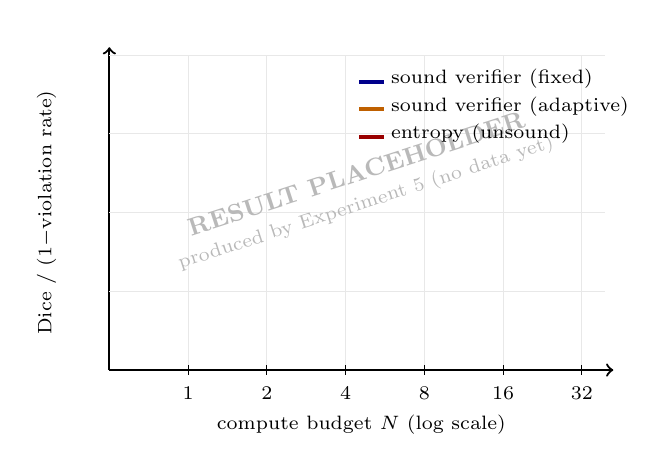
\begin{tikzpicture}[font=\small]
% axes frame
\draw[->,thick] (0,0) -- (6.4,0) node[right]{};
\draw[->,thick] (0,0) -- (0,4.1) node[above]{};
\node[rotate=90,anchor=south] at (-0.55,2.0) {\scriptsize Dice / (1$-$violation rate)};
\node[anchor=north] at (3.2,-0.45) {\scriptsize compute budget $N$ (log scale)};
% light gridlines
\foreach \x in {1,2,3,4,5,6} \draw[gray!18] (\x,0) -- (\x,4.0);
\foreach \y in {1,2,3,4} \draw[gray!18] (0,\y) -- (6.3,\y);
% x ticks for the planned budgets
\foreach \x/\lab in {1/1,2/2,3/4,4/8,5/16,6/32}
  \draw (\x,0.06) -- (\x,-0.06) node[below=1pt]{\scriptsize \lab};
% watermark: no data yet
\node[align=center,rotate=18,gray!55] at (3.2,2.3)
  {\bf RESULT PLACEHOLDER\\[-1pt]\scriptsize produced by Experiment~5 (no data yet)};
% legend stubs (no curves drawn, to avoid implying measured data)
\node[anchor=west] at (3.05,3.7) {\scriptsize \textcolor{blue!55!black}{\rule{1.1em}{1.4pt}}\ sound verifier (fixed)};
\node[anchor=west] at (3.05,3.35) {\scriptsize \textcolor{orange!75!black}{\rule{1.1em}{1.4pt}}\ sound verifier (adaptive)};
\node[anchor=west] at (3.05,3.0) {\scriptsize \textcolor{red!60!black}{\rule{1.1em}{1.4pt}}\ entropy (unsound)};
\end{tikzpicture}
\captionof{figure}{Planned compute-scaling plot (Experiment~5); axes and budgets are fixed, no data are drawn. \emph{Hypothesis to be tested}: the sound-verifier curve rises then plateaus, the adaptive schedule reaches a similar plateau at lower mean cost, and entropy selection plateaus lower or declines. We report the measured curves only after the runs return.}
\label{fig:scaling}
\end{figure}

% ============================ results ============================
\section{Results and Discussion}
\emph{This section is structured for the runs above; all numbers are placeholders until Experiments~1--5 return.}
We expect Experiment~1 to establish positive selection headroom and Experiment~2 to show the anatomical verifier recovers most of it while entropy selection does not, supporting the claim that soundness, not multiplicity of candidates, drives the gain. In Experiment~3 we expect AV-TTS to reduce the anatomical-violation rate relative to TTA baselines and, if Assumption~\ref{ass:align} holds, to improve Dice \rp{magnitudes}, with the violation-rate reduction the more directly supported effect because it is what the verifier optimizes. Experiment~5 tests whether gains follow the sound-verifier scaling shape rather than the saturating imperfect-verifier shape. If the realized gains are small, we will report that AV-TTS principally improves anatomical plausibility at modest Dice cost, and scope the contribution accordingly rather than overstate accuracy.

% ============================ limitations ============================
\section{Limitations}
AV-TTS helps only when a sound, cheap verifier exists; for lesions or pathology without a stable topological prior it reduces to base prediction by the safeguard. The guarantee in Prop.~\ref{prop:safeguard} is in the verifier metric, not Dice, and depends on Assumption~\ref{ass:align}, which we test but cannot prove. Candidate generation adds inference cost, mitigated but not removed by the adaptive schedule. Verifiers encode population-level priors and could mis-penalize rare but real anatomical variants; we report violation rates on held-out variants and recommend the safeguard with conservative tolerances in deployment.

% ============================ ethics ============================
\section*{Ethics and Responsible Use}
All datasets are public and used at test time without labels; no patient-identifying data is introduced. AV-TTS is a research method, not a clinical device; it can suppress real anomalous anatomy and must not gate diagnosis. AI tools assisted drafting; all method, proofs, and claims are verified by the human authors, who take full responsibility. The verifier-imposed priors and their failure on atypical anatomy are a fairness concern we report explicitly.

% ============================ conclusion ============================
\section{Conclusion}
Test-time scaling pays off when the verifier is sound. Medical segmentation supplies sound, label-free verifiers from anatomy, so a training-free generate--verify--select wrapper with a no-degradation safeguard is a natural and, we argue, underused route to robustness under shift. The empirical question, settled by the released runbook, is how much realized accuracy and plausibility this buys over single-pass adaptation.

\bibliographystyle{plainnat}
\bibliography{avtts_refs}

\appendix
\section{Per-benchmark verifier definitions}\label{app:verifiers}
\torun{state each penalty term, normalization, and tolerance per dataset; give the exact connected-component and Euler-characteristic implementation (see released code \texttt{avtts\_analysis.py}).}

\end{document}
